\documentclass[border=10pt]{standalone}
\usepackage{tikz}
\usetikzlibrary{arrows.meta}
\definecolor{inFill}{RGB}{183,224,177}
\definecolor{inLine}{RGB}{32,102,32}
\definecolor{hidFill}{RGB}{199,203,243}
\definecolor{hidLine}{RGB}{52,58,143}
\definecolor{outFill}{RGB}{243,199,199}
\definecolor{outLine}{RGB}{143,52,52}
\definecolor{lineC}{RGB}{38,44,110}
\begin{document}
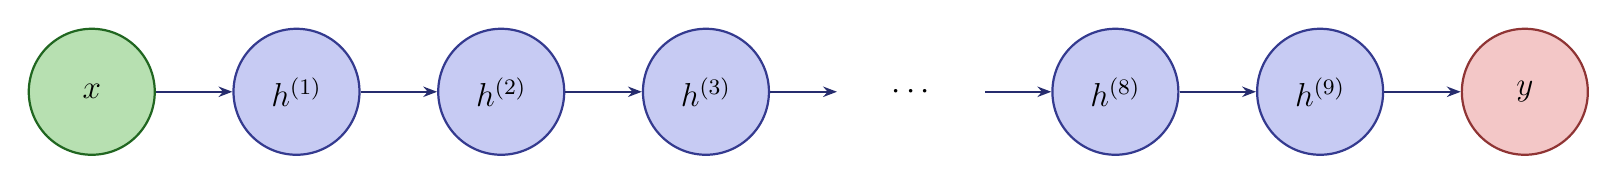
\begin{tikzpicture}[
    >={Stealth[length=5pt]}, line width=0.8pt, font=\large,
    inp/.style={circle, draw=inLine, fill=inFill, minimum size=1.6cm, inner sep=0pt},
    hid/.style={circle, draw=hidLine, fill=hidFill, minimum size=1.6cm, inner sep=0pt},
    outp/.style={circle, draw=outLine, fill=outFill, minimum size=1.6cm, inner sep=0pt},
    arr/.style={lineC, ->},
  ]
  % 单链：x → h1 → h2 → h3 → ⋯ → h8 → h9 → y
  \node[inp]  (x)  at (0,0)    {$x$};
  \node[hid]  (h1) at (2.6,0)  {$h^{(1)}$};
  \node[hid]  (h2) at (5.2,0)  {$h^{(2)}$};
  \node[hid]  (h3) at (7.8,0)  {$h^{(3)}$};
  \node       (dd) at (10.4,0) {$\cdots$};   % 省略 h4~h7
  \node[hid]  (h8) at (13,0)   {$h^{(8)}$};
  \node[hid]  (h9) at (15.6,0) {$h^{(9)}$};
  \node[outp] (y)  at (18.2,0) {$y$};

  % 链式箭头
  \draw[arr] (x) -- (h1);
  \draw[arr] (h1) -- (h2);
  \draw[arr] (h2) -- (h3);
  \draw[arr] (h3.east) -- ++(0.85,0);        % 指进省略号
  \draw[arr] (11.35,0) -- (h8.west);         % 从省略号指出
  \draw[arr] (h8) -- (h9);
  \draw[arr] (h9) -- (y);
\end{tikzpicture}
\end{document}